\section{Application Program Interface (API)}
\subsection{System}
The API is structure based on a set of micro-services on the SSM and how they relate to each other. Each micro service can be configured in specific ways and will also publish data and events to topics that relate to their capabilities and roles.
\begin{figure}[h]
    \centering
    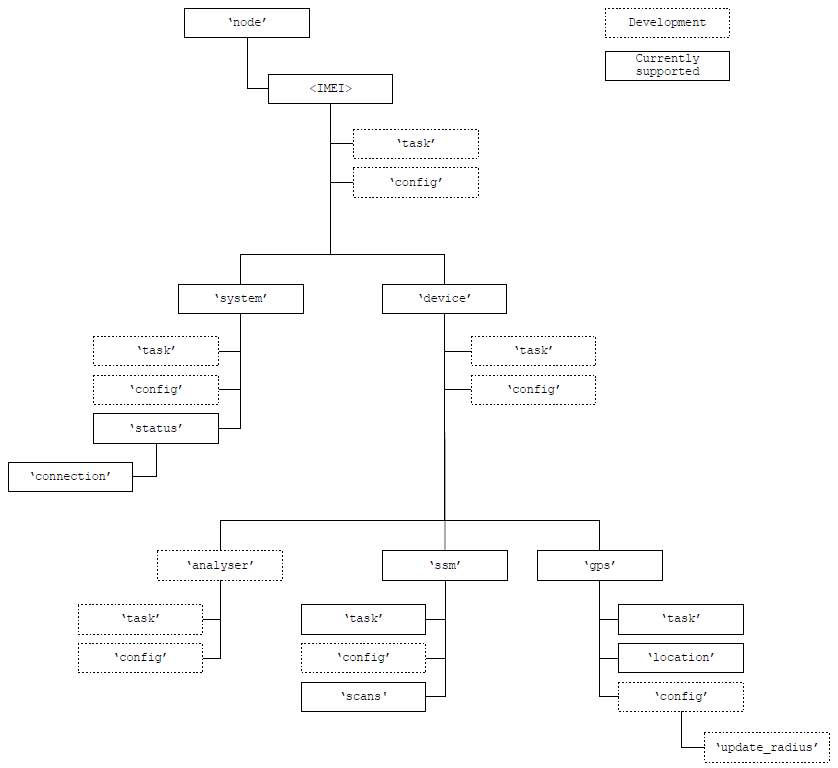
\includegraphics[width=\textwidth]{https://www.authorea.com/users/42442/articles/49215/master/file/figures/SSM/SSM.png}
    \caption{\textit{SSM MQTT service directory structure}}
\end{figure}
% ---------------------------------------------------------------------------------------------------
\subsubsection{System task interface}

Topic:
\begin{lstlisting}<IMEI>/system/task\end{lstlisting}
Type:
\begin{lstlisting}consumer\end{lstlisting}
Example response:
\begin{lstlisting}\end{lstlisting}

% ---------------------------------------------------------------------------------------------------
\subsubsection{System configuration interface}

Topic:
\begin{lstlisting}<IMEI>/system/config\end{lstlisting}
Type:
\begin{lstlisting}consumer\end{lstlisting}
Example response:
\begin{lstlisting}\end{lstlisting}

% ---------------------------------------------------------------------------------------------------
\subsubsection{Connection Status}

Topic:
\begin{lstlisting}<IMEI>/system/status\end{lstlisting}
Type:
\begin{lstlisting}producer\end{lstlisting}
    
This topic indicates whether or not the endnode is currently connected to the broker

% ---------------------------------------------------------------------------------------------------
\subsection{SSM}

\subsubsection{SSM task interface}
An XML interface to the spectrum scanner
Topic:
\begin{lstlisting}node/<I<IMEI>/ssm/task\end{lstlisting}
Type:
\begin{lstlisting}consumer\end{lstlisting}

% ---------------------------------------------------------------------------------------------------
\subsubsection{Power scans}
Topic:
\begin{lstlisting}<IMEI>/ssm/scans\end{lstlisting}
Type:
\begin{lstlisting}producer\end{lstlisting}
    
This topic outputs raw scan files

Parameters:

\begin{lstlisting}
task_id                 Task ID string 'power scan'
lower_freq              Start of the frequency range in hertz
upper_freq              End of the frequency range in hertz
bin_size                Number of FFT bins
gain                    Gain
exit_timer              Time before exiting the scan '2s'
integration_interval    Integration interval or 'dwell' "2s"
band_offset             Band offset, the amount of non-linear band to trim off (typically 20%)
\end{lstlisting}

Example:

\lstset{language=XML}
\begin{lstlisting}
<?xml version="1.0" encoding="UTF-8"?>
<task task_id="power scan" cid="jrnsljkngafdkg" lower_freq="580000000" upper_freq="590000000" bin_size="10000"  gain="30"  exit_timer="2s" integration_interval="2s" band_offset="20%"></task>
\end{lstlisting}

Output example:
\begin{lstlisting}
<scan task_id="power scan" date="2015-06-08" time="12:00:31" hz_low="580003907"  hz_high="581996093"  hz_step="9765.62" samples="224">-40.70, -41.79, -41.39, -40.56, -41.07, -41.26, -42.19, -42.18, -40.60, -41.21, -40.96, -41.99, -41.37, -41.94, -41.50, -40.38, -41.85, -40.40, -41.45, -41.90, -40.91, -40.74, -41.51, -40.98, -42.20, -41.99, -41.06, -41.72, -41.22, -41.89, -41.63, -41.87, -41.18, -41.24, -41.70, -41.62, -41.91, -42.22, -42.49, -41.70, -41.68, -41.85, -42.21, -41.80, -42.48, -42.15, -41.56, -42.15, -42.44, -42.02, -42.58, -42.44, -41.83, -41.58, -42.01, -42.35, -42.44, -41.94, -42.58, -42.35, -42.15, -42.44, -42.54, -42.55, -42.28, -42.61, -42.59, -42.08, -42.40, -42.69, -42.43, -42.31, -41.97, -41.95, -42.09, -42.69, -42.17, -42.69, -42.37, -42.19, -42.50, -42.48, -42.39, -42.34, -42.43, -42.52, -42.23, -42.18, -42.05, -42.62, -42.41, -41.87, -42.53, -42.35, -42.58, -42.01, -42.12, -42.09, -40.89, -41.16, -39.85, -40.22, -37.05, -39.15, -39.15, -40.30, -41.48, -39.99, -37.92, -37.85, -40.20, -41.50, -40.69, -38.79, -38.67, -38.58, -40.91, -39.90, -41.35, -40.21, -38.63, -40.74, -40.76, -41.48, -40.88, -40.75, -39.20, -40.83, -40.30, -41.28, -41.56, -39.71, -41.05, -40.70, -41.41, -40.88, -42.21, -40.80, -41.02, -41.15, -40.92, -41.45, -41.74, -41.40, -40.82, -41.46, -40.26, -42.21, -42.68, -41.07, -42.03, -41.21, -41.78, -41.90, -42.32, -41.74, -42.09, -41.58, -41.23, -42.76, -42.25, -42.63, -42.40, -42.32, -41.87, -42.85, -42.68, -42.27, -42.12, -41.85, -42.51, -42.34, -42.75, -42.73, -42.07, -42.07, -42.11, -42.22, -42.18, -42.42, -42.23, -42.67, -42.28, -42.49, -42.35, -42.45, -42.58, -42.11, -42.19, -42.65, -42.39, -42.89, -42.35, -42.66, -42.80, -42.71, -42.44, -43.45, -42.84, -43.52, -43.59, -42.90, -42.94, -43.12, -43.88, -43.60, -43.60</scan>
\end{lstlisting}

\subsection{Device - GPS}
\subsubsection{GPS Inbox}

Topic:
\begin{lstlisting}node/<IMEI>/gps/tasks\end{lstlisting}
Type:
\begin{lstlisting}consumer\end{lstlisting}

Example message:
\begin{lstlisting}
<?xml version="1.0" encoding="UTF-8"?>
<task task_id="location scan" cid="jrnsljkngafdkg"></task>
\end{lstlisting}



ACM0 == AT command interface 0 ( used by the dialler )
ACM1 == AT command interface 1 , used to configure and manage the modem )
ACM2 == GPS NMEA output



We have a bunch of virtual devices on the SSM module that are exposed with an
MQTT interface. Each device has an 'inbox' topic in it's root path that accepts
workflow and configuration messages (XML).

Topics:

node/<IMEI>/status
Wether or not the endnode is currently connected to the broker




    
    
    
    
    
    
    
    
    
    
    
    
    
    
    
    
    
    
    
    
    
    
    
    
    
    
    
    
    
    
  
  
  
  
  